Digital, computer-based real-time systems became widespread rapidly with the availability of microprocessors getting more powerful and cheaper from year to year.

\section{ Introduction}

Real-Time systems, as used in the wide area of automation, have 2 basic requirements,

\begin{enumerate}
	\item  The \textbf{logical correctness} of the systems output as a response to its inputs, and
	\item  The \textbf{timeliness} of the outputs available.
\end{enumerate}


For example, this is obvious for an airbag control, for which a correct decision for ignition is required at the right millisecond, otherwise the resulting behaviour can be harmful !\\

Since there is a "digital revolution" the past few decades, a strong trend to applications with microprocessors and witch microcontrollers particularly can be observed.\\

This means, that classical solutions for \textbf{real-time systems} (e.g. analog controller circuits) are replaced by \textbf{software applications} running on a microprocessor or a microcontroller.\\

Thus, an important part of \textbf{a real-time system is software}. This type of software is much different from commonly used software known from PC applications like office programs, or internet browsers, since real-time requirements have to be met.\\

In the area of real-time software development, the classical C programming language is widely used, due to its outstanding maturity and flexibility, especially with industrial PC applications, or with microcontroller applications.\\

Furthermore there is a need for PLC controls (de: SPS) in industrial automation.\\

Examples for Real-Time Systems

\begin{figure}%
    \centering
    \subfloat[\centering  Automotive Door Contol Unit with Anti-Squeeze ]{{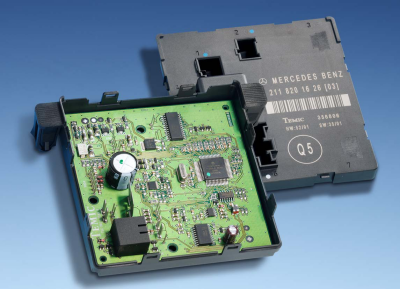
\includegraphics[width=8cm, 		   			height=5.5cm]{Images/image3.png} }}%
    \qquad
    \subfloat[\centering Undistorted image]{{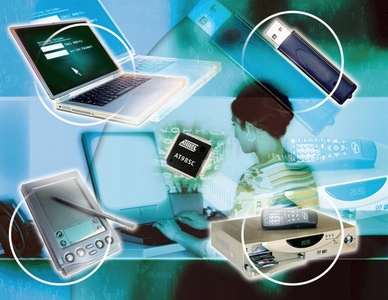
\includegraphics[width=8cm, height=5.5cm]{Images/image4.png} }}%
    \qquad
     \subfloat[\centering Car with $>$ 100 ECUs]{{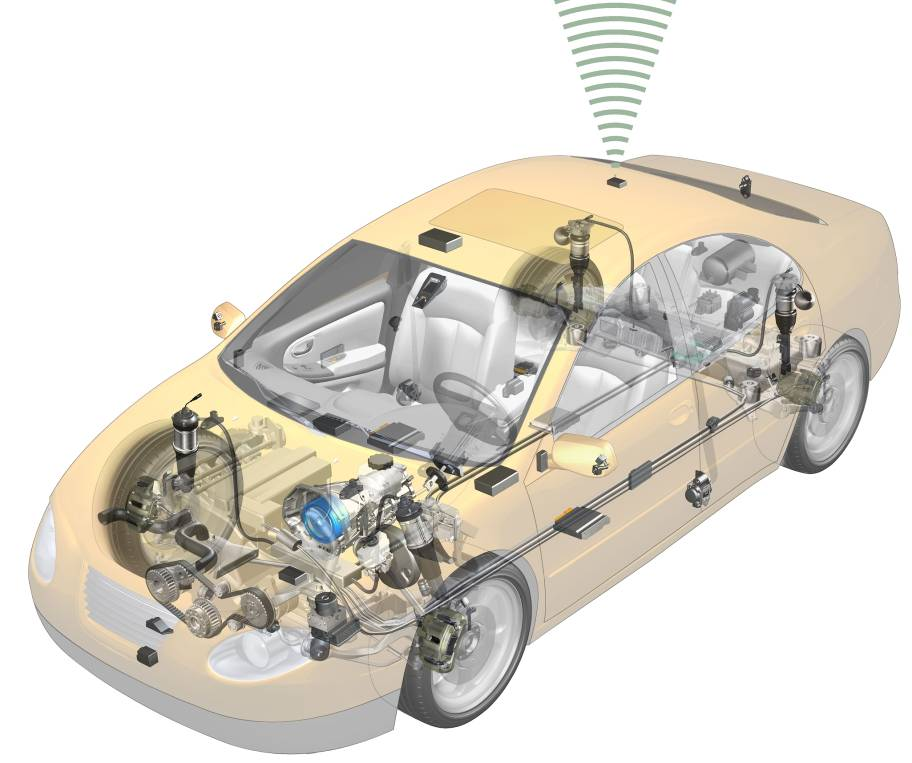
\includegraphics[width=7cm, height=5.5cm]{Images/image5.png} }}%
    \qquad
    \subfloat[\centering Pacemaker]{{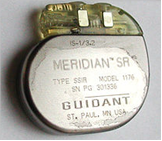
\includegraphics[width=6cm, height=5cm]{Images/image6.png} }}%
    \qquad
     \subfloat[\centering A319 Cockpit]{{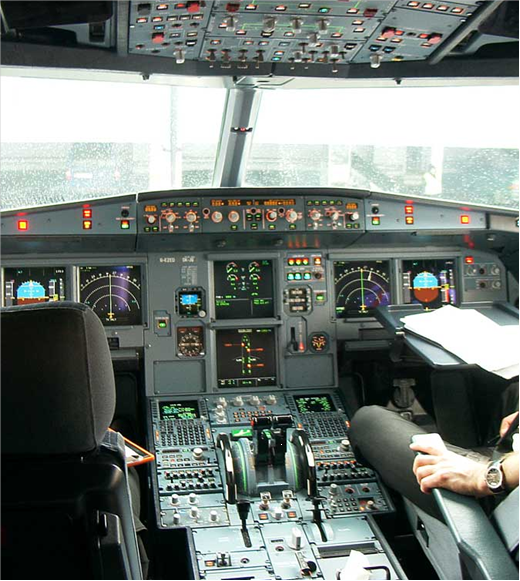
\includegraphics[width=8cm, height=5cm]{Images/image8.png}}}%
    \qquad
    \subfloat[\centering wikipedia.de: Arc welding of metal parts with industrial robots (KUKA). IPC, PLC]{{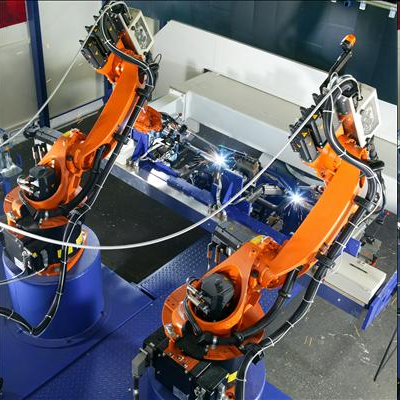
\includegraphics[width=8cm, height=5cm]{Images/image7.png} }}%
    \qquad
    \caption{ Comparison of results of video 1 (checkerboard000)}%
    \label{v1}%
\end{figure}


\begin{itemize}
	\item Examples of the use of real-time systems are found in the following areas: 
	\begin{enumerate}
		\item  Production 
		\item  Aerospace 
		\item  Automotive Electronics
		\item  Medicine
		\item  Military Technology, 
		\item  e-Banking, 
		\item  e-Trading, 
		\item  Telecommunications, 
		\item  Network Management, 
		\item  Power Generation/Management, 
		\item  Navigation
	\end{enumerate}
\end{itemize}

\textbf{The} need for Software\textbf{(mainly C-Code)in all areas of application grows rapidly}. 

\begin{tcolorbox}[colback=blue!5!white,colframe=blue!75!black]
  Moore's Law: “die Anzahl der Transistoren pro Chipfläche verdoppelt sich alle 2 Jahre”
\end{tcolorbox}

\begin{figure}[h]
    \centering
    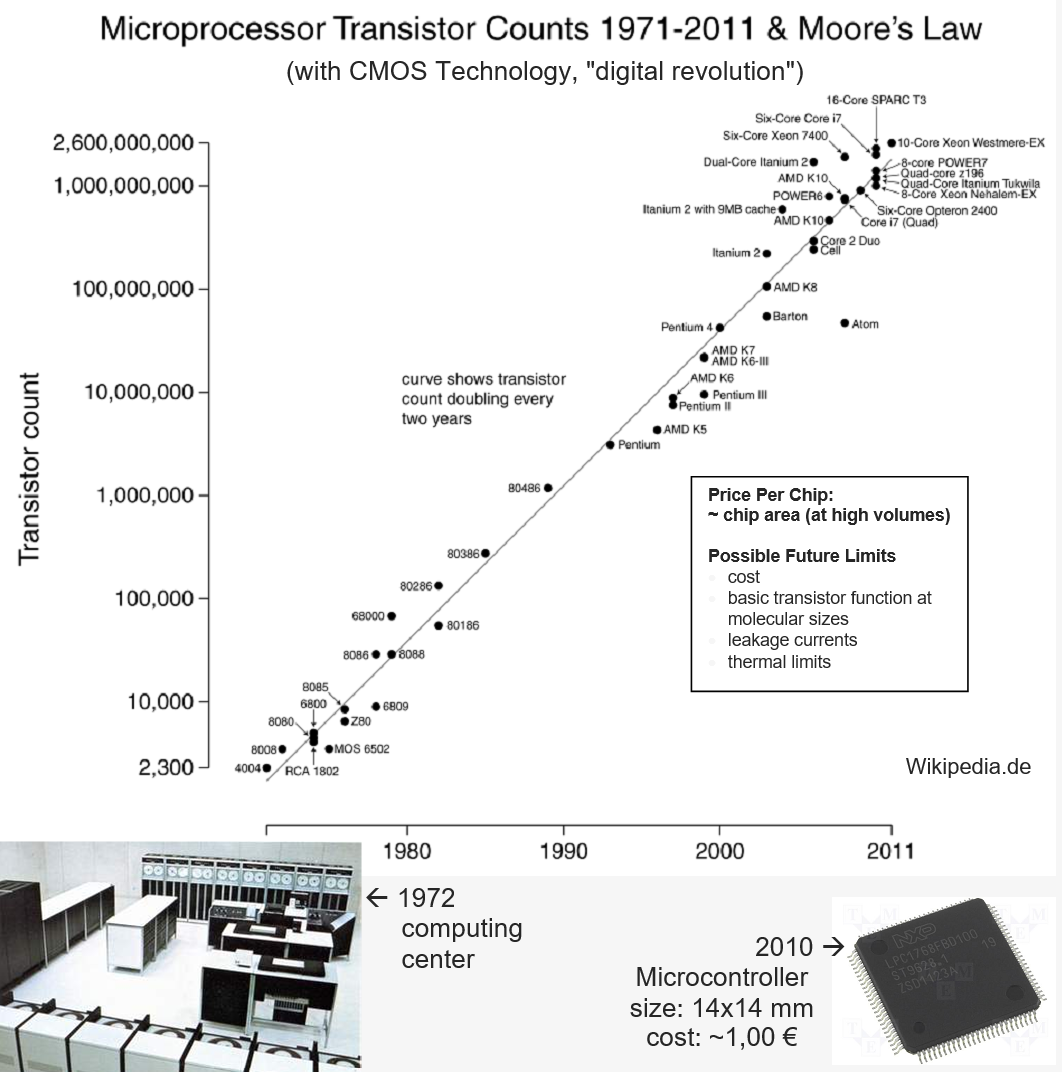
\includegraphics[width=15cm, height=11cm]{Images/image9.png}
    \caption{Moore's Law}
    \label{fig:Fig 3}
\end{figure}

\textbf{ Software for Real-Time Systems} differs substantially from software for generalpurpose computers (PC) due to the \textbf{requirements on the real-time behavior} !\\

Many methods of \textbf{classical software development} of non-real-time systems can not be used due to the lack of predictability.\\

For the development of real-time systems, special methods are required.\\
\newpage

\section{ Requirements}

The validity of an operation of a real-time system depends on

\begin{enumerate}
	\item  its logical result, and
	\item  the physical time this result is available
\end{enumerate}

\begin{figure}%
    \centering
    \subfloat[\centering logical correct, but timing incorrect]{{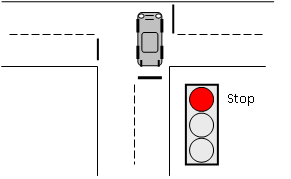
\includegraphics[width=7cm, 		   			height=5cm]{Images/image10.png} }}%
    \qquad
    \subfloat[\centering logical correct, and timing correct]{{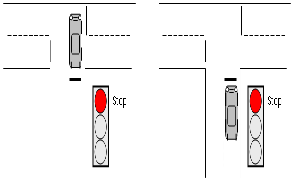
\includegraphics[width=7cm, height=5cm]{Images/image11.png} }}%
    \qquad
    %\caption{ Comparison of results of video 1 (checkerboard000)}%
    \label{fig:Fig 3}%
\end{figure}

\textbf{The traffic light control must determine traffic light phases logically and temporally correct.}\\

For real-time systems, the logical correctness \textbf{and} the timing correctness is required.

\begin{itemize}
	\item \textbf{Non Real-Time Systems}:  logical correctness  \textbf{OK}
	\item \textbf{Real-Time Systems}:    logical correctness + timing correctness  \textbf{OK}
\end{itemize}

\textbf{Example}: Real-Time Requirements with a Traffic Light Control

\begin{figure}[h]
    \centering
    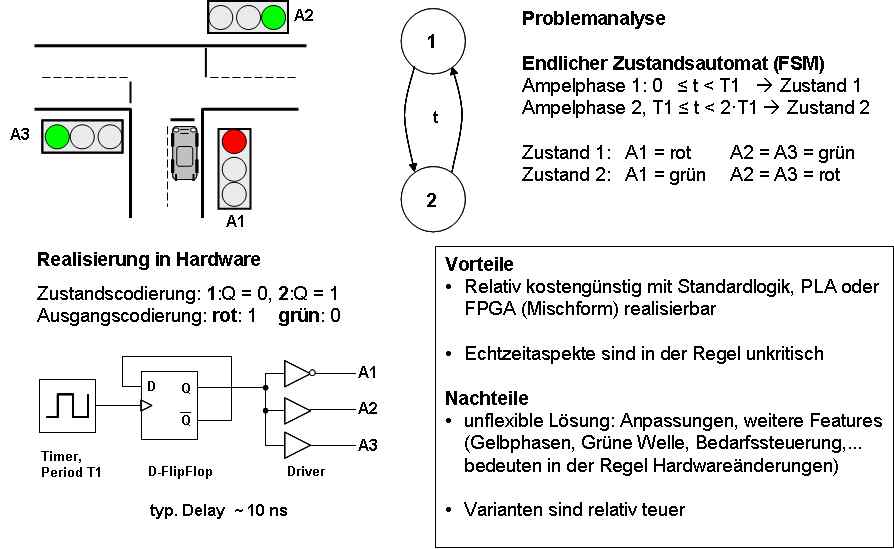
\includegraphics[width=14cm, height=9cm]{Images/image12.png}
    %\caption{Moore's Law}
    \label{fig:Fig 3}
\end{figure}

\begin{figure}[h]
    \centering
    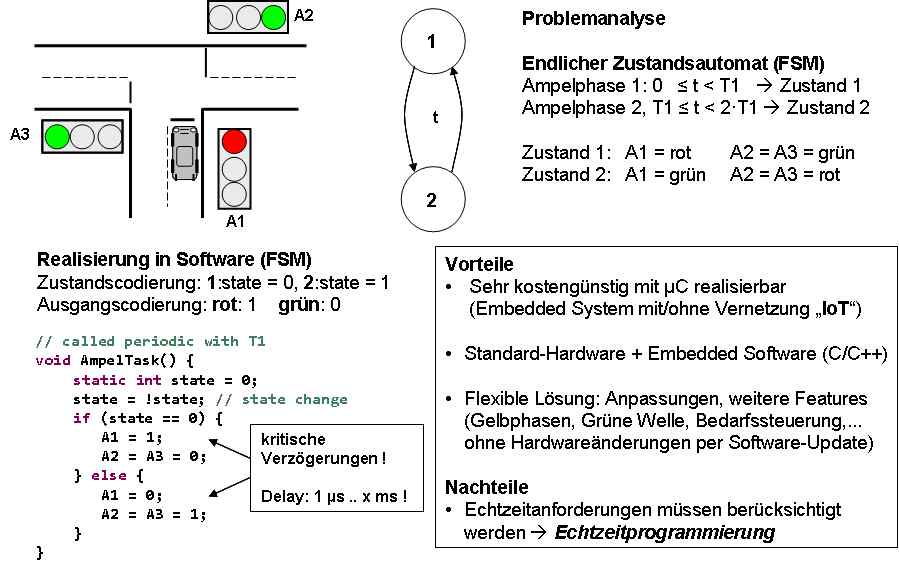
\includegraphics[width=15cm, height=9cm]{Images/image13.png}
    %\caption{Moore's Law}
    \label{fig:Fig 3}
\end{figure}

\begin{figure}[h]
    \centering
    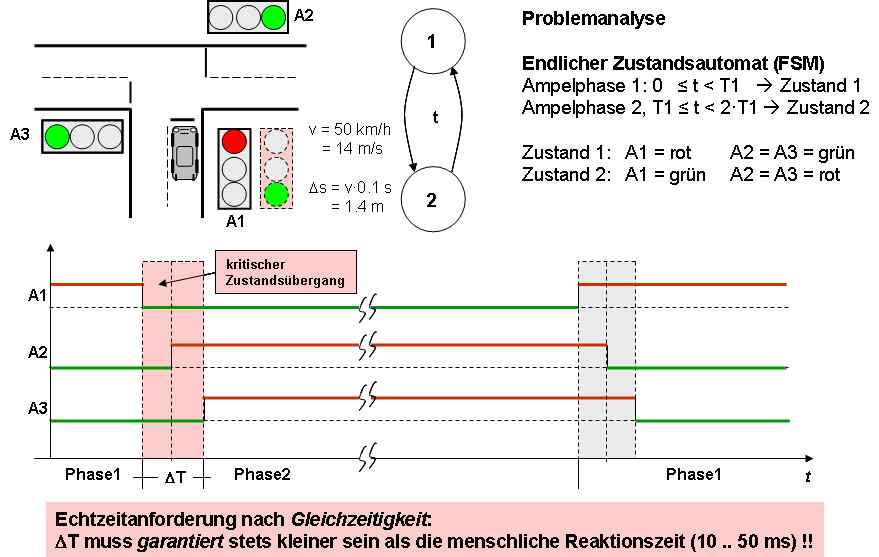
\includegraphics[width=15cm, height=9cm]{Images/image14.png}
    %\caption{Moore's Law}
    \label{fig:Fig 3}
\end{figure}

\newpage
\textbf{Solution}: Critical Section (Mutex) in AmpelTask:  see FSM Exercise\\

\begin{lstlisting}[style=mystyle, language=c]
 	// called periodic with T1  
	void AmpelTask() {
	static int state = 0;
	state = !state; // state change
  	begin(mutex);
	if (state == 0) {
		A1 = 1;
		A2 = A3 = 0;
	} else {
		A1 = 0;
		A2 = A3 = 1;
	}
  	end(mutex);
\end{lstlisting}

\newpage

{\rot\bf A Definition of Real-Time Systems is given by DIN 44300 [1985]}\\

\textit{ Realzeit-Systeme beziehungsweise Echtzeitsysteme sind Computersysteme, dieim Realzeitbetrieb arbeiten.}\\

\textit{Realzeitbetrieb wird definiert als der Betrieb eines Rechensystems, beidem Programme zur Verarbeitung anfallender Daten st\"{a}ndig betriebsbereitsind, derart, dass die Verarbeitungsergebnisse innerhalb einer vorgegebenenZeitspanne verf\"{u}gbar sind. Die Daten k\"{o}nnen je nach Anwendungsfall nacheiner zeitlich zuf\"{a}lligen Verteilung oder zu vorherbestimmten Zeitpunktenanfallen.}\\

{\rot\bf Wikipedia:}\\

In computer science, \textbf{real-time} computing (RTC), or reactive computing, is the study of hardware and software systems that are subject to a "real-time constraint", i.e., operational \textbf{deadlines} from \textbf{event to system response}. \\

By contrast, a \textbf{non-real-time system}  is one for which there is \textbf{no deadline}, even if fast response or high performance is desired or preferred. \\

The needs of real-time software are often addressed in the context of real-time operating systems, and synchronous programming languages, which provide frameworks on which to build real-time application software.\\

A real time system may be one where its application can be considered (within context) to be mission critical. \\

The anti-lock brakes on a car are a simple example of a real-time computing system - the real-time constraint in this system is the short time in which the brakes must be released to prevent the wheel from locking. \textbf{Real-time computations} can be said to have \textbf{failed if} they are \textbf{not completed before their deadline}, where their deadline is relative to an event. \\

\textbf{A real-time deadline must be met, regardless of system load}.\\

Thus, in a real-time system the logical correctness (functional correctness) of the answers with guaranteed response times (temporal correctness) is of essential importance. \\

The temporal behavior in real-time systems is part of the system specification and thus subject of the product verification.\\

\textbf{Embedded systems} often have to meet \textbf{real-time requirements}.\\

{\rot\bf Technical Process and Process Model}\\

A technical process can be defined as follows (DIN 66 201):

In a technical process materials, energy or information (the process media) are converted or transported (such as an end product) into grafted materials, energy or information. \\

Its input and state variables summarized in the vector \textbf{Z} can be measured with sensors and controlled by actuators: \\

\begin{figure}[h]
    \centering
    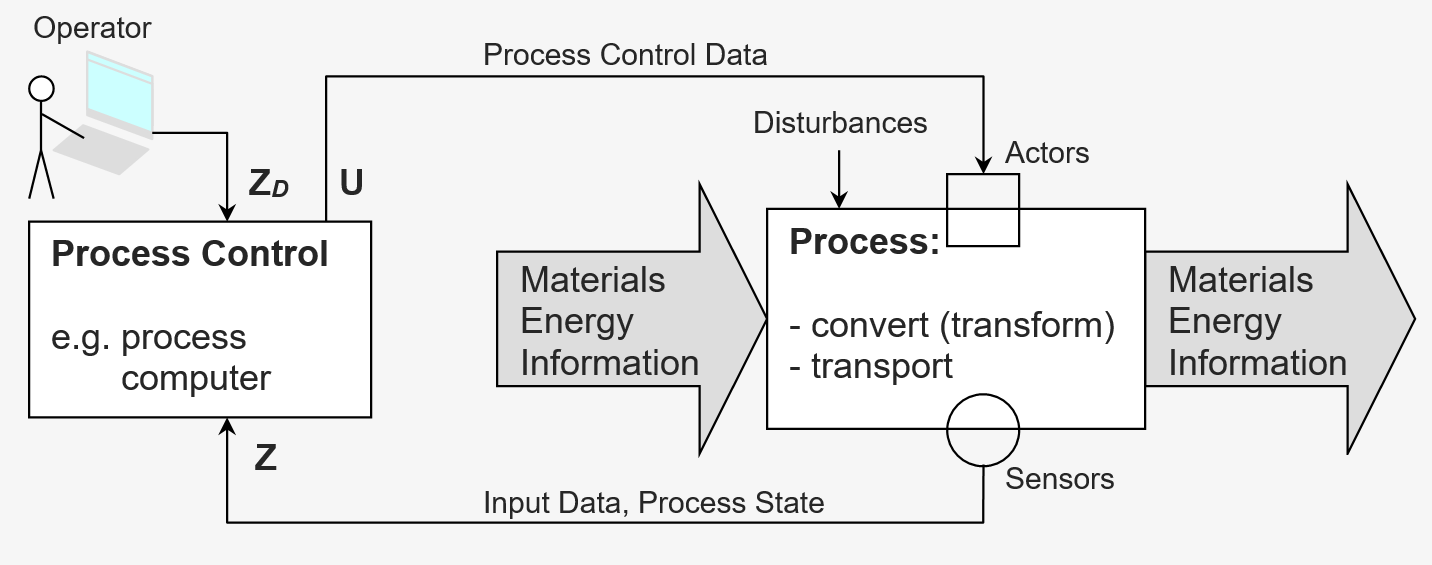
\includegraphics[width=14cm, height=6cm]{Images/image60.png}
    %\caption{Moore's Law}
    \label{fig:Fig 3}
\end{figure}

In automation, the process is controlled via control actions (vector \textbf{U}) so that after a given time, a desired process target or a desired state \textbf{Z\textit{${}_{D}$}} is reached. \\

The desired state can refer to the following:

quality, quantity (of the final product), speed, stability, security (during the transforming process), production, yield, raw material consumption, emissions, or even reaching the next process step (e.g. with sequential processes).\\

The delay time in the loop is of \textbf{\textit{crucial importance}} for the \textbf{\textit{stability}} of the \textbf{\textit{entire system}}!

This delay time must therefore be exactly specifiable  \textbf{\textit{Real-Time Programming}} !\\

{\rot\bf Timeliness}\\

The timeliness (=timing correctness) is directly derivable from the above considerations requirement for all real-time systems. For digital process computers timing correctness is, the output data must be calculated in time.\\

This also requires that the input data must be collected on time. The timing deadlines, and are usually given by a technical process:\\

\begin{figure}[h]
    \centering
    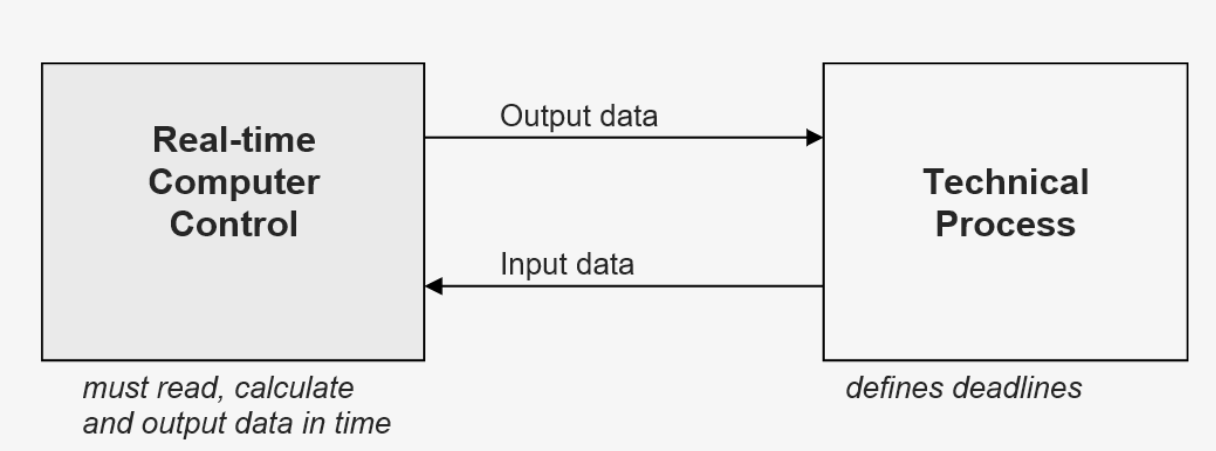
\includegraphics[width=12cm, height=5cm]{Images/image61.png}
    %\caption{}
    \label{fig:Fig 3}
\end{figure}

Thus the allowed response time for the controller is limited to a known value, thus real-time systems are said to be \textbf{predictable} or \textbf{deterministic}.\\

Input data must be read in time for a real-time system, and the output data to be generated must be provided within the given deadline (time condition). \\

The primary requirement for a real-time control is the \textbf{constant ability to input, process and output data on time regardless of the system workload}.\\ 

For a real-time system also means that it \textbf{monitors the temporal validity} of information and prevents the use of invalid data !\\

This must apply regardless of whether the data to be processed are \textbf{event based} or at \textbf{predetermined (e.g. periodic) times}.\\

However, due to complexity, the timing behavior of real-time systems \textbf{can never be predicted with 100~\% certainty}  System validation by tests !\\

{\rot\bf Time Conditions}\\

The \textbf{time conditions} to monitor, and control a process can be in several variants

\begin{enumerate}
\item  A precise time \textit{t}${}_{0}$ for a controller action is defined. This action must not be executed earlier or later.
	
	\begin{figure}[h]
    \centering
    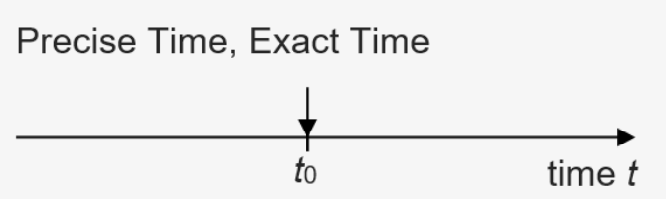
\includegraphics[width=6cm, height=1.5cm]{Images/image62.png}
    %\caption{}
    \label{fig:Fig }
	\end{figure} 

\textbf{Examples}: Sampling Systems (DSP \& Digital Control),      clock display control.

\item  A maximum time \textit{t}${}_{max}$ (=deadline) for a controller action is defined. This action must be finished latest at its deadline, but it can be finished earlier. 

	\begin{figure}[h]
    \centering
    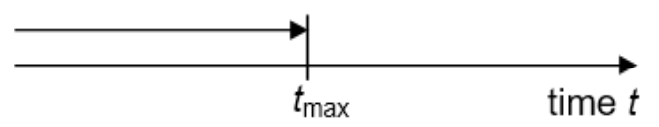
\includegraphics[width=6cm, height=1.5cm]{Images/image63.png}
    %\caption{}
    \label{fig:Fig }
    \end{figure}
    
\textbf{Examples}: a sampling system calculating an output sample for the next sampling      period, Anti-Squeeze Control, maximum response time with switching      on/off a machine, UI control reaction time to a button, slider, {\dots}      e.g. \textit{t${}_{max}$} $\mathrm{<}$ 50ms with human reaction times  "\textit{immediately}"    

\item  Earliest Time Limit A minimum time \textit{t}${}_{min}$ for a controller action is defined. The action must not be executed earlier, but it can be executed later. 
	
	\begin{figure}[h]
    \centering
    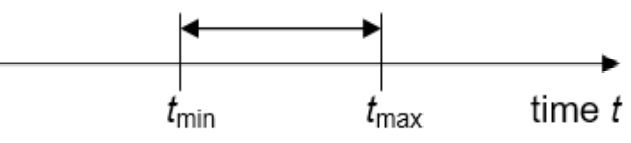
\includegraphics[width=6cm, height=1.5cm]{Images/image64.png}
    %\caption{}
    \label{fig:Fig }
    \end{figure}
    
\textbf{Examples}: transitions in state machines, an output may not occur before a state       transition has been finished.

\item  Time IntervalAn action must be executed within a time interval [\textit{t}${}_{min}$, \textit{t}${}_{max}$], thus at any time earlier than \textit{t}${}_{max}$ and later than\textit{ t}${}_{min}$. 

	\begin{figure}[h]
    \centering
    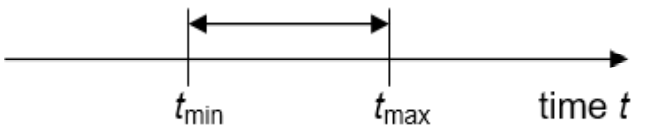
\includegraphics[width=6cm, height=1.5cm]{Images/image65.png}
    %\caption{}
    \label{fig:Fig }
    \end{figure}

\textbf{Example}:  airbag ignition in some crash situations an airbag shall be ignited      e.g. 10-30 ms, in other situations 5-8 ms after crash.
\end{enumerate}

Time conditions can be \textbf{periodic} or \textbf{non-periodic}. \\

{\rot\bf Periodic Time Condition }\\

A periodic time condition is given with analog signals to be sampled and processed by a digital computer. Any analog signal has to be discretized in both value and time by a constant periodic sampling time \textit{T}${}_{s}$. This is typical for sampling systems realizing digital filters or digital control algorithms for processing quasi analog signals.

	\begin{figure}[h]
    \centering
    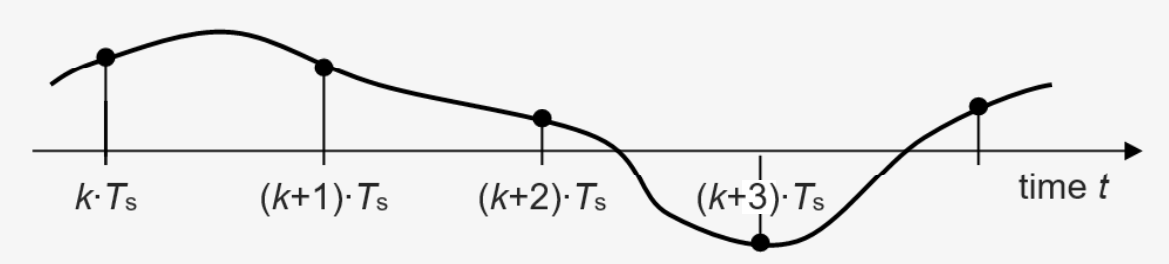
\includegraphics[width=12cm, height=4cm]{Images/image66.png}
    %\caption{}
    \label{fig:Fig }
    \end{figure}

An example is the electric signal of a microphone which has to be sampled \textbf{strictly periodic} in order to have a \textbf{digital representation} of the \textbf{original analog sound signal}. Any deviation from the periodic sampling results in unwanted noise, which cannot be compensated. After time sampling the values of the voltage signal is discretized by an AD-Converter.\\

{\rot\bf Sampling Theorem [Kamm], [Oppen]}

\begin{tcolorbox}[colback=blue!5!white,colframe=blue!75!black]
  The basic theorem of Shannon / Kotelnikov in signal theory states, that any analog signal x(t), which is sampled at constant frequency fs can be perfectly reconstructed from the sampling series x(k.Ts), apart from a constant delay, if the signal bandwidth Bx is not larger than half the sampling frequency fs = 1 / Ts, so Bx $<$ fs / 2.
\end{tcolorbox}

\textbf{Example}: CD-Audio: \textit{f}${}_{s}$ = 44.1 kHz, \textit{T}${}_{s}$ = 22.7 µs  \textit{B${}_{x}$} = 20 kHz $\mathrm{<}$ 0.5 \textit{f}${}_{s}$ = 22.05 kHz \\

Correct sampling:       tagesschau\_44.1.wav \\
Sampling theorem violation:  tagesschau\_D10.wav\\

Digital signal processing of analog signals involves very strict requirements to real-time conditions, due to the periodic and exact sampling conditions.\\

\begin{tabular}{|p{2.2in}|p{1.9in}|} \hline 
\textbf{Action} & \textbf{Time Condition} \\ \hline 
input of a sample of an analog signal    & exact periodic sampling at  k$\mathrm{\bullet}$\textit{T}${}_{s}$ \\ \hline 
computation of a signal sample  & time interval [k$\mathrm{\bullet}$\textit{T}${}_{s}$ + \textit{T${}_{ADC}$,} (k+1)$\mathrm{\bullet}$\textit{T}${}_{s}$] \\ \hline 
output of the calculated signal sample & exact periodic sampling at  (k+1)$\mathrm{\bullet}$\textit{T}${}_{s}$ \\ \hline 
\end{tabular}
\newpage

{\rot\bf Non-Periodic Time Condition}\\

A non-periodic time condition is given frequently with digital signals to be processed at arbitrary, non-predictable times due to events like pushing or releasing a switch or a revolution sensor, producing a slope at discrete angles of a motor shaft.\\

	\begin{figure}[h]
    \centering
    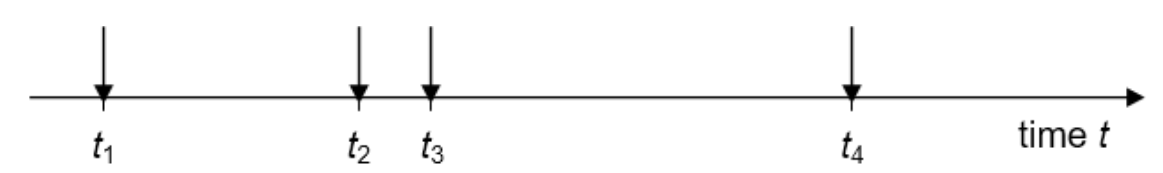
\includegraphics[width=12cm, height=1.5cm]{Images/image67.png}
    %\caption{}
    \label{fig:Fig }
    \end{figure}

\textbf{Absolute Time Condition }\\
With an absolute time condition defined, an action must be executed at a certain global time, i.e. an action must be performed at 12:00:00 MEZ.\\

\textbf{Relative Time Condition }\\
With a relative time condition defined, an action must be executed relative to some previous event. Example: a control signal must be updated after 0.5~s after a push button was pressed.\\

All time conditions can arise in combinations.For meeting the time conditions a real-time system must have

\begin{enumerate}
	\item  \textbf{sufficient processing speed} to process the input and output data at the required speed (sampling frequency), which the technical process requires
	\item  \textbf{deterministic time behavior}
\end{enumerate}

\subsection{Hard and Soft Real-Time Systems}

In the previous section, we saw that computation must complete before reaching a given deadline. In other words, real-time systems have timing constraints and are deadline-driven. Real-time systems can be classified, therefore, as either hard real-time systems or soft real-time systems.\\

What differentiates hard real-time systems and soft real-time systems are the degree of tolerance of missed deadlines, usefulness of computed results after missed deadlines, and severity of the penalty incurred for failing to meet deadlines.\\

For \textbf{hard real-time systems}, the level of tolerance for a missed deadline is extremely small or zero tolerance. The computed \textbf{results after} the \textbf{missed} \textbf{deadline} \textbf{are} likely \textbf{useless} for many of these systems. The penalty incurred for a missed deadline is \textbf{catastrophic} (e.g. an unstable control loop). \\

For \textbf{soft real-time systems}, however, the level of tolerance is non-zero. The computed \textbf{results after} the \textbf{missed deadline} have a \textbf{rate of depreciation}. The \textbf{usefulness} of the results does \textbf{not reach zero immediately} passing the deadline, as in the case of many hard real-time systems. The physical impact of a missed deadline is\textbf{ non-catastrophic}.

\begin{enumerate}
	\item  \textbf{Hard Real-Time Conditions} \\
	The time conditions must be met, or catastrophes occur !  Deviations from the time-conditions are not allowed and represent a serious error. In safety-related systems a violation of the hard real-time time conditions can endanger human life (e.g. if sampling controls become unstable). Systems, meeting the hard real-time conditions are called \textbf{\textit{Hard Real-Time Systems}}.\\
	
\textbf{Examples}: Sampling Controls (closed-loop), aerospace flight controls, airbag ignition, automotive X-by-wire, pacemakers, {\dots} 
	\item  \textbf{Soft Real-Time Conditions} \\
	The deadlines must be met but with a degree of flexibility. The deadlines can contain varying levels of tolerance, average timing deadlines, and even statistical distribution of response times with different degrees of acceptability. A missed deadline does not result in system failure, but costs can rise in proportion to the delay, depending on the application. Systems meeting soft real-time conditions are called \textbf{\textit{Soft Real-Time Systems}}.\\
	
\textbf{Examples}: multimedia-streams (speech, video, music, low level audio), toasters, refrigerators, {\dots} 
\end{enumerate}

\subsection{Concurrency}

Real-time systems must generally treat multiple inputs and outputs simultaneously. Thus, the simultaneous addition to the timeliness of the second general requirement for real-time systems.\\

Example is about a CNC machine tool, where the x-y axes must be controlled simultaneously (synchronously, concurrently) to move the tool along a predetermined path \textit{B}(\textit{x}, \textit{y}) = \textit{B}(\textit{x}(\textit{t}), \textit{y}(\textit{t})). 

	\begin{figure}[h]
    \centering
    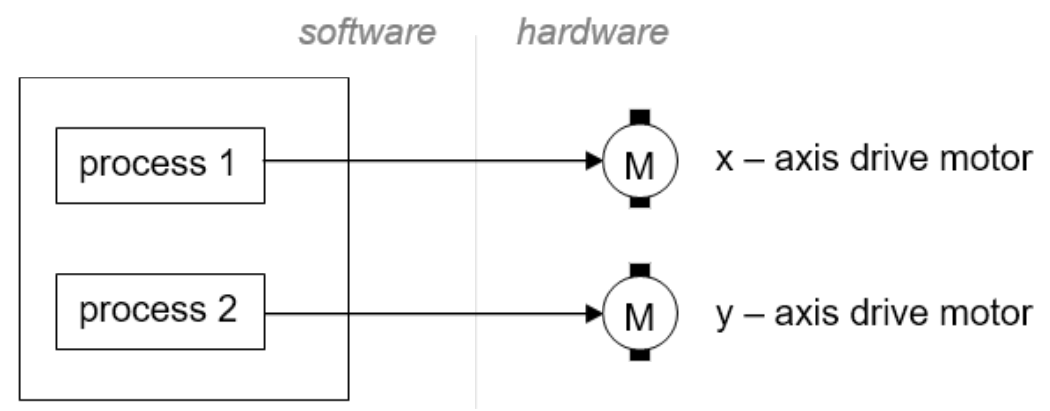
\includegraphics[width=12cm, height=5cm]{Images/image68.png}
    %\caption{}
    \label{fig:Fig }
    \end{figure}

There is an relative time condition for both processes acting concurrently on the two drive axes x and y:

	\begin{figure}[h]
    \centering
    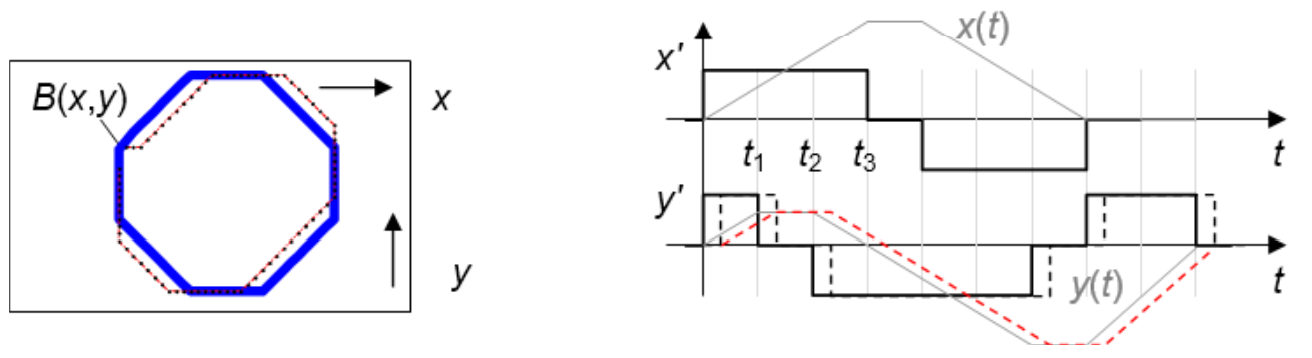
\includegraphics[width=14cm, height=5cm]{Images/image69.png}
    %\caption{}
    \label{fig:Fig }
    \end{figure}

If the time axis of x and y are shifted by some amount of time $\Delta$\textit{T} (e.g. due to different clocks for x- and y-drive control), the resulting path \textit{B}(\textit{x}, \textit{y}) = \textit{B}(\textit{x}(\textit{t}), \textit{y}(\textit{t-}$\Delta$\textit{T})) will be wrong.\\

\textbf{Example}: Tolerances {\textbar}\textit{x}{\textbar}, {\textbar}\textit{y}{\textbar} $\mathrm{<}$ 0.05 mm,   Requirement    \textit{v${}_{x}$} = \textit{v${}_{y}$} = \textit{x}' = \textit{y}' = $\mathrm{\pm}$10 cm/s     Requirement     {\textbar}\textit{t}{\textbar} $\mathrm{<}$ {\textbar}\textit{x}{\textbar} / {\textbar}\textit{v${}_{x}$}{\textbar} = 0.5 ms       Synchronization, Real-Time Condition

\subsection{ Realizations of Real-Time Systems with Concurrency Requirement}

To meet the requirement of concurrency, there are several possibilities:

\begin{enumerate}
	\item  Full parallel processing in a multiprocessor system
	\item  Quasi-parallel processing in a multiprocessor system
	\item  Quasi-parallel processing in a uniprocessor system (\textbf{Multitasking})
\end{enumerate}

	\begin{figure}[h]
    \centering
    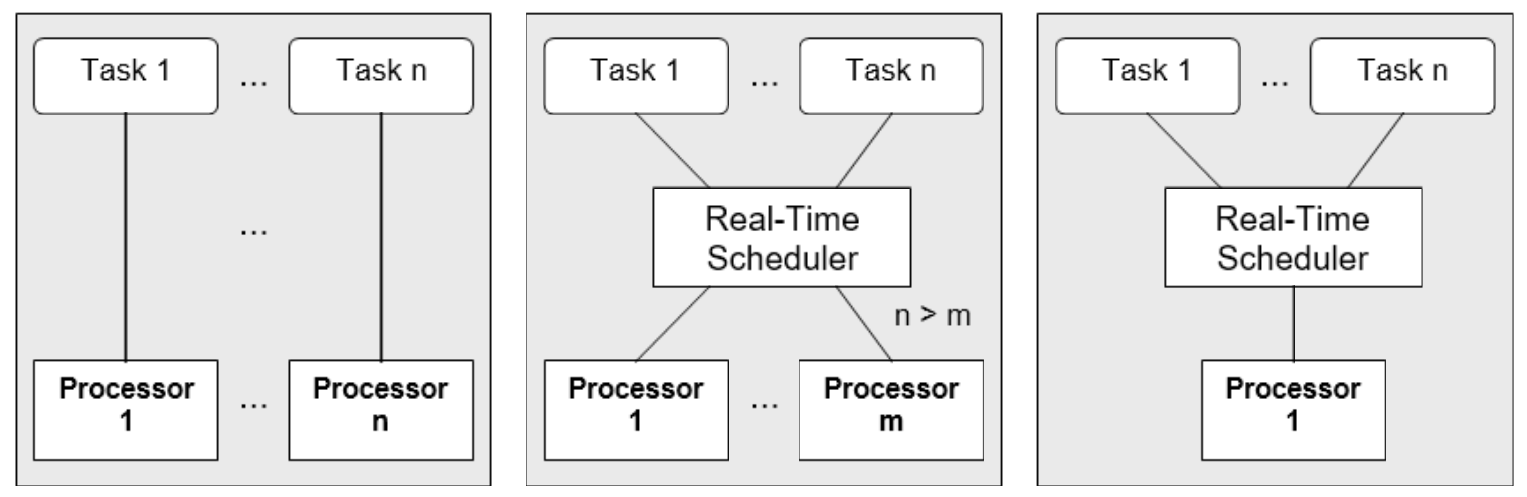
\includegraphics[width=15cm, height=6cm]{Images/image70.png}
    %\caption{}
    \label{fig:Fig }
    \end{figure}
    
Each task is processed on a separate processor (e.g. microcontroller). There is a real parallel processing, each task has the full power of its own processor. This allows the independent consideration of each task, however, the tasks must be synchronized in most cases (e.g. x-y axis control of the CNC machine).\\

Each task executed on a processor that is allocated by a real-time scheduler(there are usually fewer processors available than tasks). The real-time scheduler is a hardware or software component, which assigns the tasks to processors such that all tasks can meet their timing constraints.The individual tasks can be assigned to single processors.\\

From a hardware perspective, the simplest and most cost effective and realization: All tasks share a single processor \textbf{Multitasking}. A Real Time Scheduler controls the allocation of the processor to the task. This form of real-time scheduling is the easiest to analyze and control \\ 

$\rightarrow$ preferred realization of most embedded systems.\\

{\rot\bf  Availability: }\\

Real-time systems must be available without interruption, otherwise time conditions may be violated. This leads to the third basic requirement of real-time systems, the \textbf{availability}. \\

Real-time systems must be available over a longer period of time, maybe around the clock without any breaks, as with

\begin{itemize}
	\item  Power Plant Controls
	\item  Production Facilities
	\item  Heating and Air Conditioning Systems
	\item  Communication
	\item  Medical Applications ...
\end{itemize}

This requires that there is no disruption of operations for phases of system reorganization. A typical example here is the garbage collection of some programming languages such as Java or C \# or their runtime environments. \\

For example, the default Java implementation is not suitable for use in real-time systems. 

	\begin{figure}[h]
    \centering
    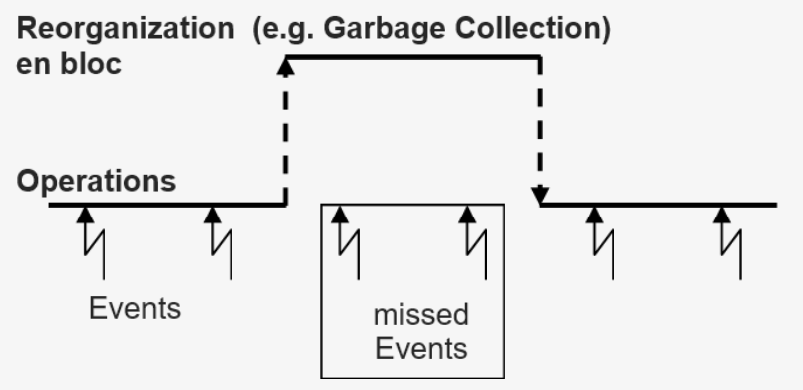
\includegraphics[width=10cm, height=4cm]{Images/image71.png}
    %\caption{}
    \label{fig:Fig }
    \end{figure}

Remedy is the use of algorithms free of need for reorganization (such as for dynamic memory management).\\

\textbf{Example }: Algorithm for Calculation of a Factorial in C 

	\begin{figure}[h]
    \centering
    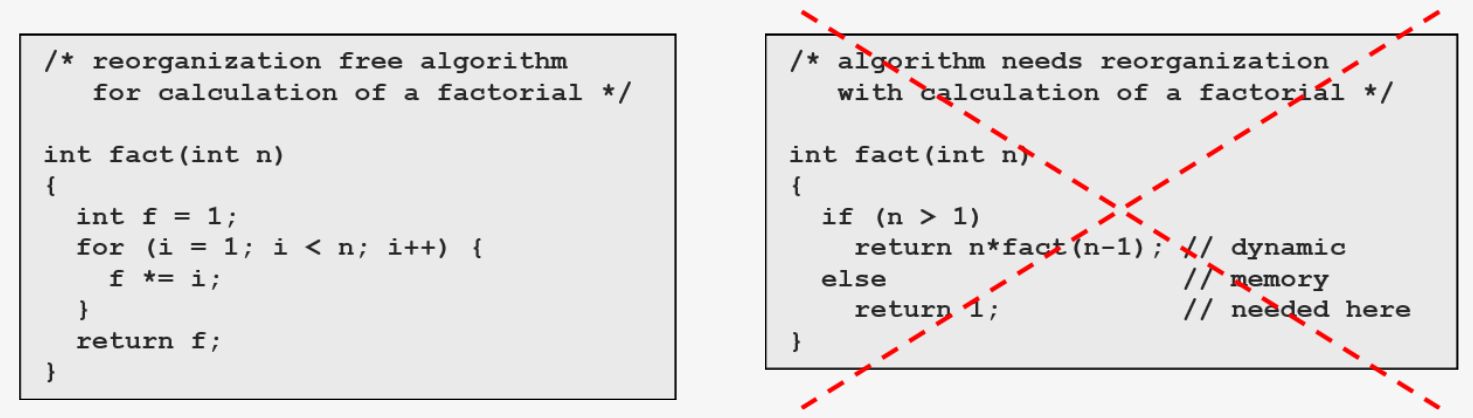
\includegraphics[width=15cm, height=5.5cm]{Images/image72.png}
    %\caption{}
    \label{fig:Fig }
    \end{figure}

OK with Real-Time programming   \hspace{1.5cm}   Not OK with Real-Time programming ! (Exec.-Time of stack  operations not deterministic due to recursion). \\


Another possibility is to divide the reorganization into small steps under control of the real-time scheduler to ensure that no time constraint is violated: 

	\begin{figure}[h]
    \centering
    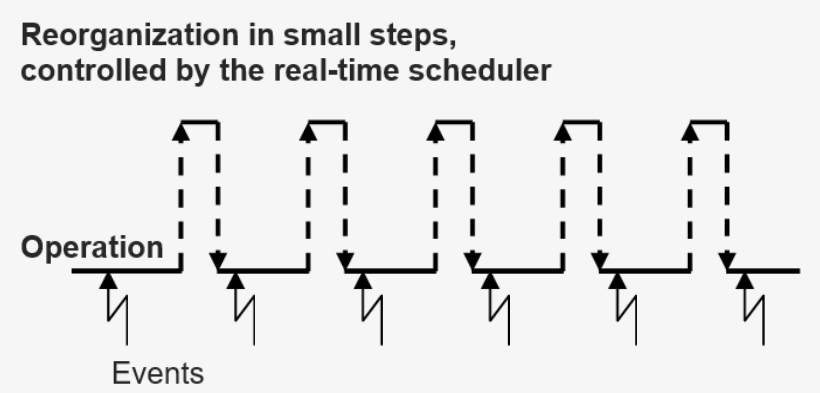
\includegraphics[width=10cm, height=5cm]{Images/image73.png}
    %\caption{}
    \label{fig:Fig }
    \end{figure}
\newpage
This method is been used by Real-Time Java (Real-Time Specification for Java (RTSJ)).Also, more traditional memory management strategies involve not predictable time for execution (like \textbf{malloc/free} of the C standard library, \textbf{new/delete} with C++)\\

$\rightarrow$ dynamic memory management is typically avoided with hard real-time systems !\\

\textbf{Example}:

	\begin{figure}[h]
    \centering
    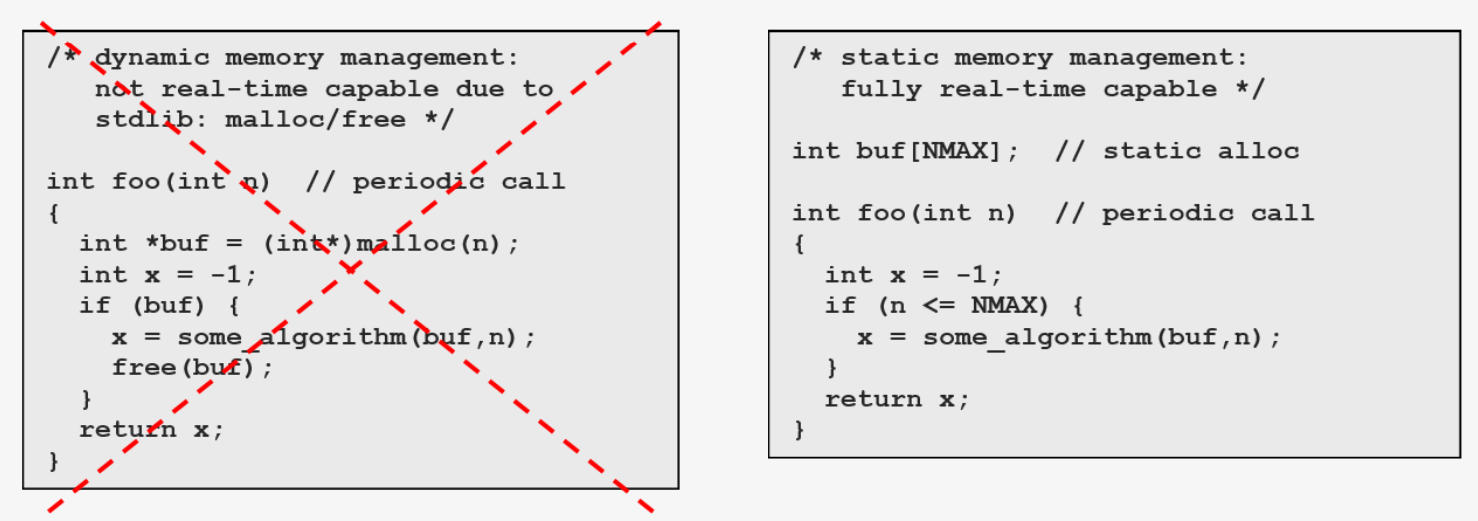
\includegraphics[width=15cm, height=5cm]{Images/image74.png}
    %\caption{}
    \label{fig:Fig }
    \end{figure}
    
Not OK with Real-Time programming   \hspace{3cm}  OK with Real-Time programming !\\
(Exec.-Time of malloc() non deterministic)\\
- but: malloc() in initialization possible  

\section{Timing Definitions}

{\rot\bf Process Time and Processing Time}\\

The time interval between two requests of the same type is called the \textbf{process time} \textit{T${}_{P}$}. If the interval between two events is constant, it is called a periodic event. In many cases, however, the time interval varies, so that there is a time interval with a minimum \textit{T${}_{Pmin}$} and a maximum \textit{T${}_{Pmax}$}.\\

For the actual processing of the event computer instructions (operations) have to be executed. The event belongs to the sequence of instructions is referred to as the code sequence or a job. Jobs are implemented within the computer as a computational process, which can be distinguished as \textbf{tasks} and \textbf{threads} (see section \textbf{Process Management}). \\

For the execution of a job i the computer needs \textbf{processing time} \textit{T${}_{Vi}$} (from de: \textit{Verarbeitungszeit}) which is also called \textbf{execution time}.\\

The \textbf{processing/execution time }needed for a certain number of operations \textit{N} is inverse to the \textbf{computing power} \textbf{\textit{P}} (in ops / sec) a processor core (CPU) offers:

\begin{equation}
	Tv = N / P \hspace{3cm} [Tv] = ops / (ops / sec) = sec
\label{EQ 1}
\end{equation}

The CPU power is approximately proportional to the CPU clock frequency.\\

In practice it is not easy to specify the processing/execution time for a certain task, since it often depends on the input values (conditional branches). Furthermore, the performance of the processor varies (due to caches, pipelines and DMA). To calculate \textit{T${}_{Vmax}$} in real-time systems, \textit{N${}_{max}$} and \textit{P${}_{min}$} shall be used in \ref{EQ 1}.

	\begin{figure}[h]
    \centering
    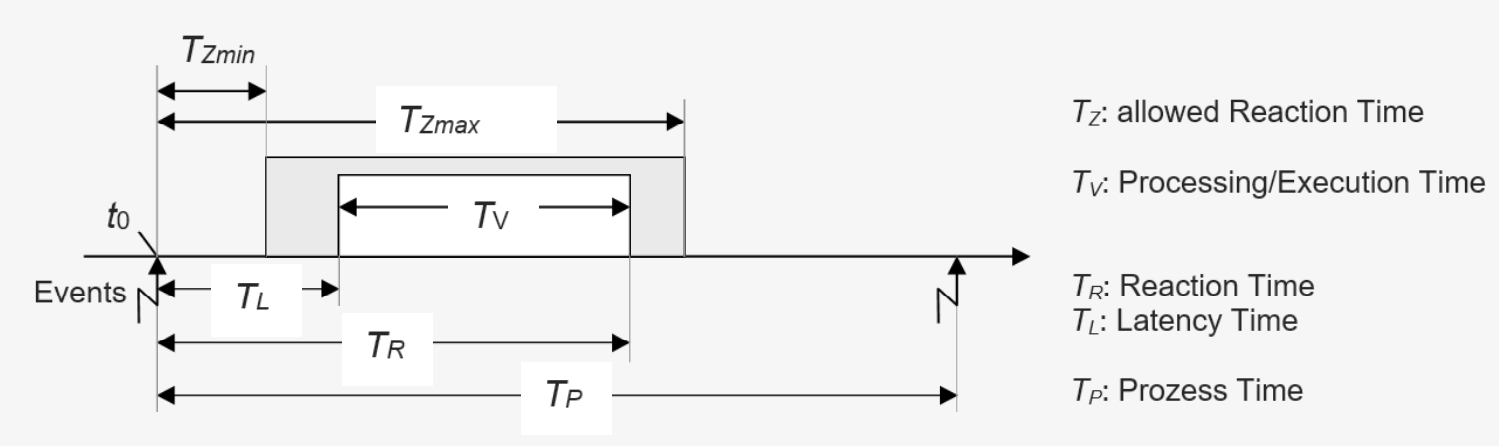
\includegraphics[width=15cm, height=5cm]{Images/image75.png}
    %\caption{}
    \label{fig:Fig }
    \end{figure}

\textbf{Timeliness, Response time and Maximum Response Time}\\

Timeliness means, that a task required at the time \textit{t}${}_{0}$\\
\hspace{3cm} is done \textbf{not before} a specified time \textit{t}${}_{0}$ + \textit{T${}_{Zmin}$} and\\
\hspace{3cm} is done \textbf{no later} than a specified time \textit{t}${}_{0}$ + \textit{T${}_{Zmax}$} (timeliness).\\

The requirement for a minimum latency, i.e, that a task is not been done before a certain time, is often missing (\textit{T${}_{Zmin}$} = 0) or can be realized easily.\\ 

On the other hand, the requirement for \textbf{timeliness} (\textit{T${}_{R\ }$}$\mathrm{<}$ \textit{T${}_{Zmax}$}) is hard to guarantee. \\

The \textbf{maximum reaction time} \textit{T${}_{Rmax}$} is the worst-case time when task execution ends and the computer can cause a reaction. \\

The \textbf{maximum reaction time} \textit{T${}_{Rmax}$} always needs to be \textbf{smaller} than the \textbf{maximum response time} \textit{T${}_{Zmax}$}.\\

{\rot\bf Utilization, Load}\\

The computer core (CPU, processor) is loaded (utilized) depending on the frequency of occurrence of an event. The utilization  gives a relative measure how much the CPU is loaded by a task is the quotient of the necessary processing time \textit{T${}_{V}$} and process time \textit{T${}_{P}$}

\begin{equation}
	\rho = Tv/Tp
\label{EQ 2}
\end{equation}
	
The total utilization ${}_{ges}$ is the sum of the utilization of all individual jobs \ref{EQ 3}. A real-time system must be able to process all tasks with fulfilling their requirements for timeliness -- this is sometimes referred to as the requirement for concurrency (in a wider sense).\\

 Mathematically, this means that the total utilization \textit{${\rho}_{ges}$} is less than 100\%:

\begin{equation}
	\begin{array}{l} {\rho _{ges} =\sum _{i=1}^{n}\rho _{i} = \sum _{i=1}^{n}\frac{T_{Vi} }{T_{Pi} }  } \\ {\rho _{ges} <\, \, 1} \end{array}
\label{EQ 3}
\end{equation}

\section{Real-Time Evidence}

Evidence that all time requirements of all requests are met under all conditions, is very difficult (practically impossible). \\

In principle, the real-time evidence is based on

\begin{enumerate}
	\item  evaluate the relevant characteristics of the technical process,
	\item  number of different requirements
	\item  Minimum processing time for each request
	\item  Minimum allowable response time for each request \textit{T${}_{Zmin}$}
	\item  Maximum allowable response time for each request \textit{T${}_{Zmax}$}
	\item  dependencies between events
	\item  identify the maximum processing time \textit{T${}_{VMax}$} (WCET = Worst Case Execution Time) for each request
	\item  check the\textbf{ load condition} (\ref{EQ 3})
	\item  verify the \textbf{timeliness condition} (determination of \textit{T${}_{Rmin}$} and \textit{T${}_{Rmax}$}).
\end{enumerate}

With verifying the \textbf{timeliness condition} in particular, it is not trivial to determine the maximum response time \textit{T${}_{Rmax}$}.\\

{\rot\bf Estimate for the Worst Case Execution Time (WCET)}\\

The maximum processing time \textit{T${}_{VMax}$} -- often called Worst Case Execution Time (WCET) -- of a request is very difficult to determine. The WCET depends in particular on the algorithm, the implementation of the algorithm, the hardware used and the other activities of the system (other computing processes). \\

Therefore, the WCET at best be estimated. In principle, two methods for determining the WCET can be distinguished:

\begin{enumerate}
	\item  measure the WCET 
	\item  static code analysis with WCET determination (count operations,cycle).
\end{enumerate}

{\rot\bf WCET Measure}\\

The WCET is determined by execution of the code sequence that will be processed, normally on the target platform. The time between the onset of the event and output at the end of the code sequence is determined.\\
 
Condition: Modification of the real-time software

	\begin{figure}[h]
    \centering
    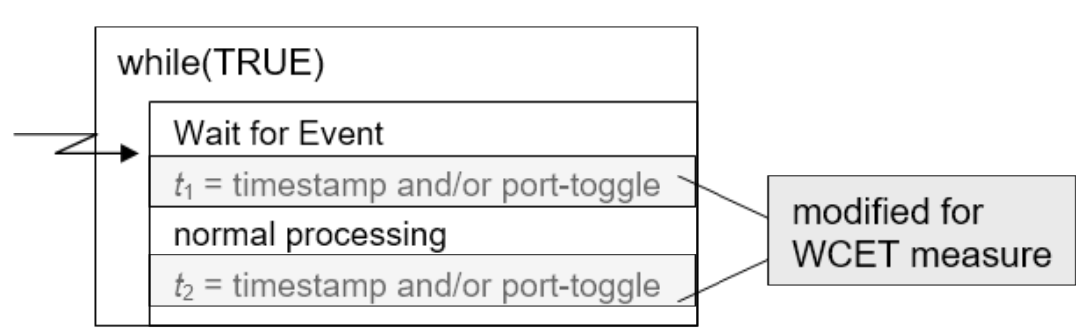
\includegraphics[width=10cm, height=5cm]{Images/image76.png}
    %\caption{}
    \label{fig:Fig }
    \end{figure}
\newpage

\textbf{Method for Measuring WCET}\\

To measure this time can be divided into two basic methods:\\


1st Measurement by the measure out piece of code itself (see above).The piece of code will be amended such that every time an event arrives and when the reaction took place, a time stamp\textit{ t}${}_{1}$ ( free running timer) is stored. At the end of the code, a second time stamp\textit{ t}${}_{2}$ is stored.\\
$\rightarrow$ the difference \textit{T${}_{Vi}$} = \textit{t}${}_{2}$ - \textit{t}${}_{1}$ is the actual execution time.\\
	
The first value \textit{T${}_{V}$}${}_{1}$ is stored as \textit{T${}_{Vmax}$}. With subsequent iterations, a newly calculated time \textit{T${}_{Vi}$}  is compared with the stored value. If the newly calculated time is greater than the previously measured WCET, the new value overwrites the existing WCET\\
	
\textit{T${}_{Vmax}$} = max(\textit{T${}_{Vi}$})\\

External measurement of event and response (output), by means of an oscilloscope using port-toggle.

	\begin{figure}[h]
    \centering
    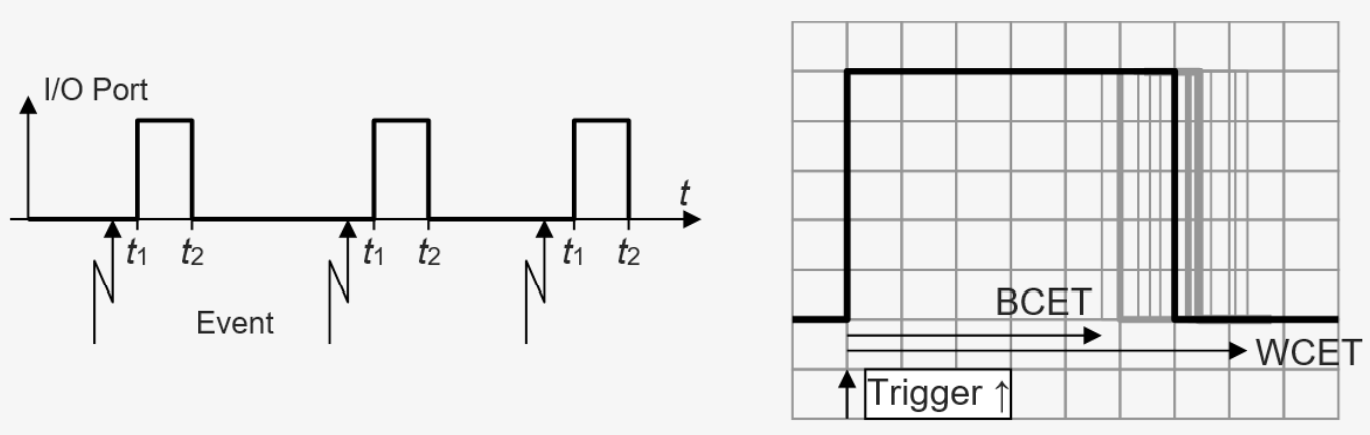
\includegraphics[width=15cm, height=5cm]{Images/image77.png}
    %\caption{}
    \label{fig:Fig }
    \end{figure}
    
For a WCET measure, appropriate input values and events must are generated. In addition, the entire system must be put under load (e.g. by an automatic tester).\\

\textbf{Advantages} of the method:

\begin{enumerate}
	\item  Independent of a programming language
	\item  Relatively easy to implement
	\item  Can run as autonomous self-diagnosis
\end{enumerate}

\textbf{Disadvantages} of the method:\\

\begin{itemize}
	\item  The WCET of a code sequence can not be guaranteed, after all, it depends on many factors (background, loop iterations, caches, branches, etc ..).
	\item  The measurement is WCET is time consuming and ultimately expensive. Measure out the piece of code needs to be theoretically charged with all input data (in any combination).
	\item  This method can be carried out with the running code on the target platform only. Thus, an assessment at an early stage of development can be difficult.
	\item  A test environment is required (which provides the input data to create).
	\item  The code sequence to be measured out must be modified (for storing time stamps) $\rightarrow$ \textbf{timers}.
	\item  It is sometimes difficult to put the system under the required load.
\end{itemize}

\subsection{Static Code Analysis}

Here, the code itself is analyzed. Therefore most often an analysis tool program is used, which is fed with the object (machine) code, rather than with the C-source code. In addition, a hardware description is necessary (e.g. clock frequency of the micro-controller). \\

The tool allows the duration of each code sequences to be estimated. After that, the number of loop iterations are considered, a bound of the number of cycles and the estimated execution time \textit{T${}_{SA}$} is printed.\\

Analysis can get rather complex, if cache hits, cache misses, processor pipelining are conssidered. \\

If there are safety requirements, the code measured is not to changed after a static code analysis.\\

As a safety margin factors of \textit{c} = 2, 3, sometimes are used to state an upper limit\\

\textit{t}${}_{Vmax}$ $\mathrm{\le}$ \textit{T${}_{SA}$ }· \textit{c}\\

A manual determination of the number of cycles can be done in simple cases by inspection of the C-compiler generated assembler code:\\

Example: timer-interrupt routine for AVR microcontroller (e.g. ATmega8\_sum.pdf).

	\begin{figure}[h]
    \centering
    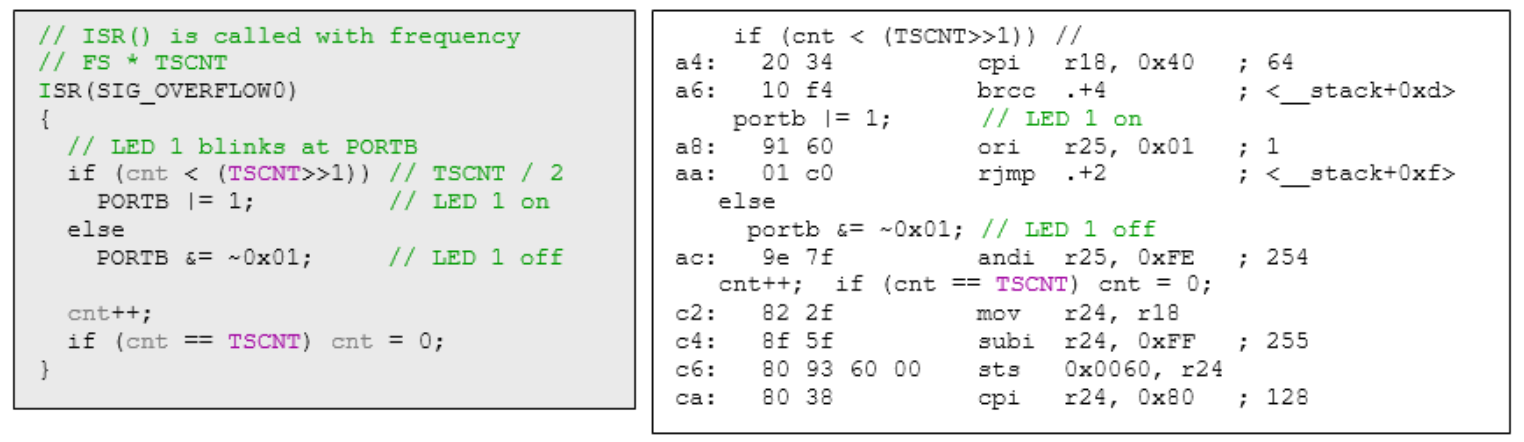
\includegraphics[width=17cm, height=5.5cm]{Images/image78.png}
    %\caption{}
    \label{fig:Fig }
    \end{figure}
    
The C-compiler generated assembly-/machine-code, ultimately determines the number of cycles to complete a section of code for a particular microcontroller (AVR here). The number of cycles multiplied by the instruction cycle time is the execution time.\\

{\rot\bf Estimation of the Best Case Execution Time (BCET)}\\

The determination Best Case Execution Time of a job can be done as the WCET, with the least possible load on the system, which can be easily implemented in general-at least in a test environment.\\

\textit{T${}_{Vmin}$} = min(\textit{T${}_{Vi}$})

